\subsection{2026-09-21 --- EDA round 3: how should the data be transformed?}
\label{sec:eda-round-3}

Rounds 1--2 asked what is in the data and what makes the problem hard. This round asks the
engineering question: \emph{given tree models, which transformations actually create signal?}
Full notebook: \texttt{src/EDA/eda\_round3.ipynb}.

\subsubsection*{A framing constraint that prunes the search space.}
Trees are invariant to monotonic transforms of a \emph{single} column --- rescaling, logging or
min-max normalising one feature does nothing at all to an XGBoost model. Only transforms that
\emph{combine} information can help, and there are exactly four such families: column
combinations (differences, ratios), time-window aggregates, graph/space aggregates, and
cross-sectional ranks. All feature work should come from those four.

\subsubsection*{Correcting the ``noise ceiling'' claim from round 2.}
Section~\ref{sec:eda-round-2} measured that labels are 12\% self-inconsistent and inferred an
``effective ceiling on achievable accuracy''. The measurement stands; \textbf{the inference was
wrong}, in two specific ways. First, it conflated a label-flip rate with an AUC ceiling --- AUC
is a \emph{ranking} metric, and a model can rank well-ordered probabilities highly even where it
would be wrong at a 0.5 threshold. Second, it assumed the horizon boundary condition was
unobservable; it is not, and is quantified below. External evidence that scores around 0.99 are
attainable on this dataset is consistent with the disagreement being \emph{signal we are not
capturing} rather than noise.

\subsubsection*{Normalisation: which component creates the signal?}

\begin{figure}[htbp]
  \centering
  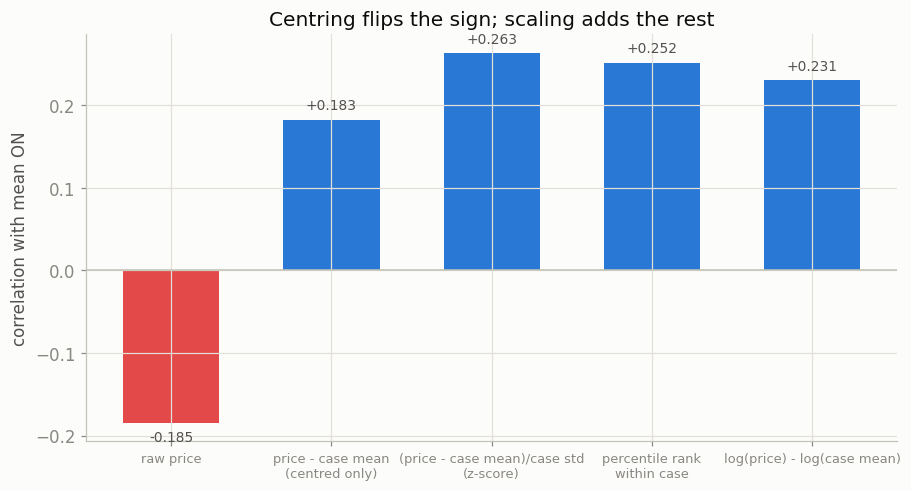
\includegraphics[width=0.78\linewidth]{figures/eda3_01_normalisation_components.png}
  \caption{Correlation with mean ON for five price transformations.}
  \label{fig:eda3-norm}
\end{figure}

\finding{\textbf{(1)} Raw price correlates $-0.185$ with commitment; subtracting the case mean
flips it to $+0.183$; dividing by the case's own standard deviation reaches $+0.263$
(Figure~\ref{fig:eda3-norm}). The two operations do different jobs: \textbf{centring removes the
cross-period scarcity confound} (high-price years are scarce-water years) and \textbf{scaling
makes a $\pm5$ EUR deviation in 2015 comparable to a $\pm100$ EUR deviation in 2022}. Percentile
rank within the case ($+0.252$) captures nearly all of it distribution-free. \emph{Price features
should be case-relative and scale-free, never raw levels.}}

\finding{\textbf{(2)} The opposite rule holds for the price\,$-$\,water-value spread: raw
$+0.241$ vs.\ z-scored within case $+0.114$. The spread is \emph{already} relative --- price
measured against its own opportunity cost --- so normalising twice destroys the cross-case level
information. \textbf{Normalise price; do not normalise the spread.}}

\subsubsection*{The optimizer is forward-looking.}

\begin{figure}[htbp]
  \centering
  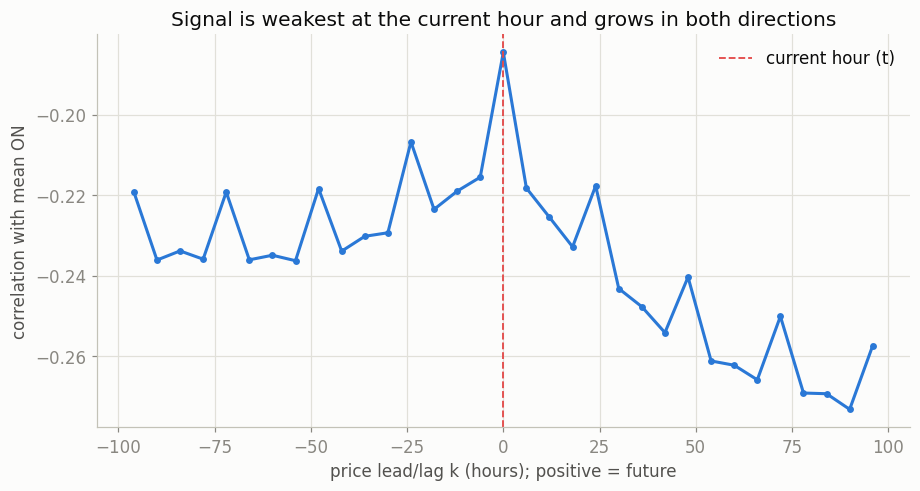
\includegraphics[width=0.78\linewidth]{figures/eda3_02_price_lead_lag.png}
  \caption{Correlation between mean ON and price at lead/lag $k$.}
  \label{fig:eda3-leadlag}
\end{figure}

\finding{\textbf{(3)} The price/commitment correlation is \textbf{weakest at the current hour}
($-0.185$ at $k=0$) and strengthens in \emph{both} directions, peaking around $k=+90$h
($-0.273$) --- see Figure~\ref{fig:eda3-leadlag}. The optimizer uses the whole horizon, and the
\emph{sustained level} of price over multi-day windows matters more than the instantaneous value.
Forward-looking window features are legitimate here because the full 168h price path is known at
solve time.}
\supersededby{sec:eda-round-3b}{this curve ignored case boundaries; the corrected peak is $\approx-0.245$, and the ``legitimacy'' claim is refined there.}

\subsubsection*{Dimensionality and graph structure.}

\begin{figure}[htbp]
  \centering
  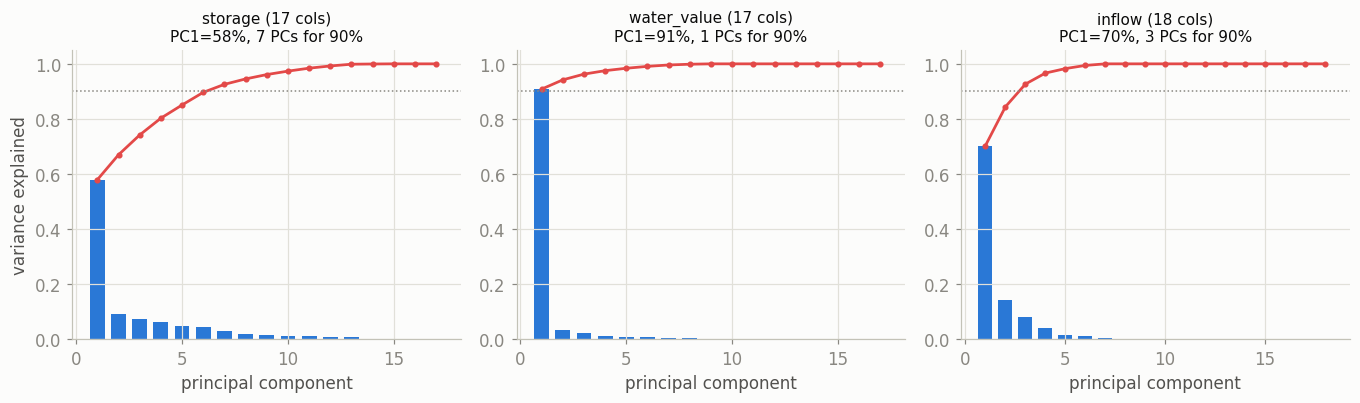
\includegraphics[width=0.95\linewidth]{figures/eda3_03_pca_dimensionality.png}
  \caption{Variance explained by principal components within each feature family.}
  \label{fig:eda3-pca}
\end{figure}

\finding{\textbf{(4)} The 17 water-value columns have \textbf{PC1 $=$ 91\%} of variance --- they
are effectively \emph{one} system-wide scarcity factor (Figure~\ref{fig:eda3-pca}). Inflow needs
3 components for 90\%, storage 7. Adding more per-reservoir water-value columns is near-useless;
the informative decomposition is \textbf{(system common factor) $+$ (reservoir-specific
deviation)}.}

\begin{figure}[htbp]
  \centering
  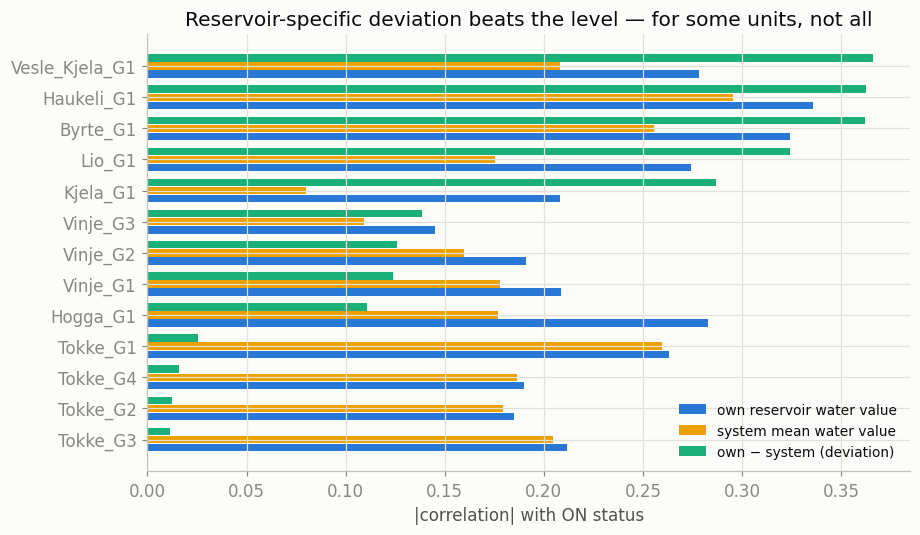
\includegraphics[width=0.78\linewidth]{figures/eda3_04_graph_aggregation.png}
  \caption{Own-reservoir vs.\ system-mean vs.\ own-minus-system water value, per unit.}
  \label{fig:eda3-graph}
\end{figure}

\finding{\textbf{(5)} The \textbf{own $-$ system} water-value deviation is the strongest of the
three for Vesle\_Kjela\_G1 (0.366 vs.\ 0.278), Byrte\_G1, Haukeli\_G1, Kjela\_G1 and Lio\_G1, but
is $\sim$0.01 for the Tokke units because Vinjevatn tracks the system almost perfectly
(Figure~\ref{fig:eda3-graph}). Graph/neighbourhood features help \emph{selectively and per unit}
--- which a single global feature set cannot express.}

\subsubsection*{The unused boundary condition.}

\begin{figure}[htbp]
  \centering
  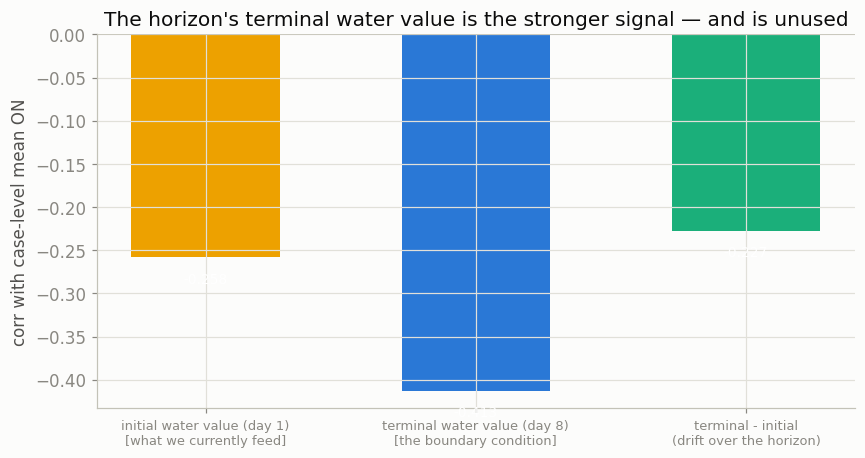
\includegraphics[width=0.72\linewidth]{figures/eda3_05_terminal_water_value.png}
  \caption{Initial vs.\ terminal horizon water value against case-level commitment.}
  \label{fig:eda3-terminal}
\end{figure}

\finding{\textbf{(6)} The dataset documentation states a case's \emph{final} water value is the
value at start $+$ 8 days. We feed the model the \textbf{initial} value and never the terminal
one. The terminal value correlates $\mathbf{-0.41}$ with case-level commitment versus $-0.26$ for
the initial value, and the two differ in \textbf{93\%} of case/reservoir pairs
(Figure~\ref{fig:eda3-terminal}). A genuine per-case boundary condition, documented in the data
and entirely unused.}

\subsubsection*{Two hypotheses tested and refuted.}

\begin{figure}[htbp]
  \centering
  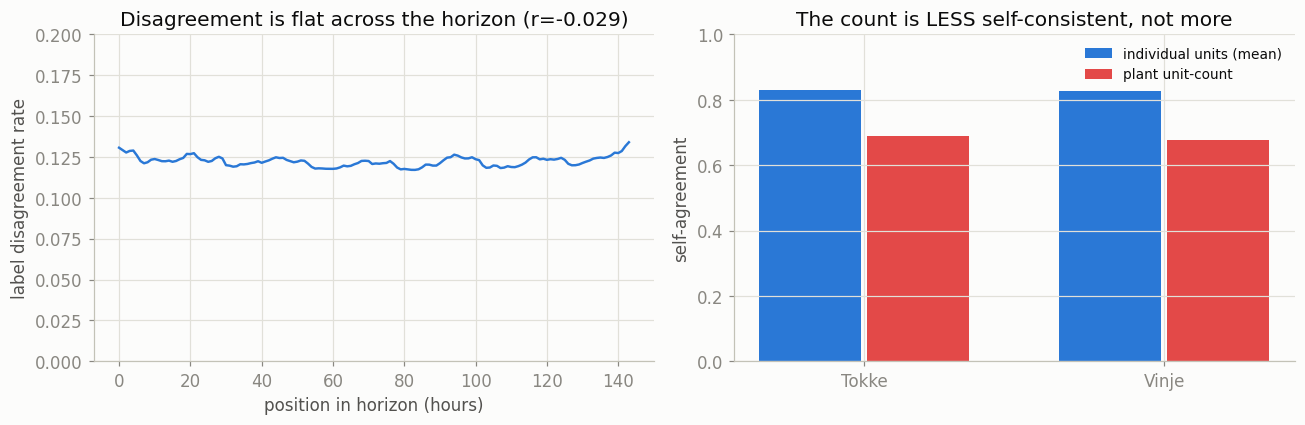
\includegraphics[width=0.95\linewidth]{figures/eda3_06_refuted_hypotheses.png}
  \caption{Left: disagreement vs.\ horizon position. Right: unit vs.\ count self-agreement.}
  \label{fig:eda3-refuted}
\end{figure}

\finding{\textbf{(7, refuted)} I expected label disagreement to concentrate at the end of the
horizon where the boundary condition bites. It is \textbf{flat} ($r = -0.03$). The terminal water
value shapes the whole week's schedule, not just its tail. \emph{No horizon-position sample
weighting is justified.}}

\finding{\textbf{(8, refuted)} I predicted per-plant \emph{counts} would be less noisy than
individual units. They are \textbf{more} noisy (Tokke 0.688 vs.\ 0.829) --- obvious in hindsight,
since a sum disagrees whenever any term does. This does not invalidate the count-based
architecture from Section~\ref{sec:eda-round-2}, but its justification is the merit-order
determinism, \emph{not} a noise reduction. Claim corrected.}

\subsubsection*{Transformation rules established.}
\begin{itemize}
  \item Price features: case-relative and scale-free (z-score or percentile), never raw levels.
  \item The price\,$-$\,water-value spread: use raw, do \emph{not} normalise.
  \item Use multi-day forward \emph{and} backward price windows, not the current hour.
  \item Water value: one common factor plus deviations, not 17 correlated columns.
  \item \texttt{own $-$ system} deviations help selectively, per unit.
  \item Feed the terminal (day-8) water value alongside the initial one.
  \item No horizon-position weighting; counts are not a noise reduction.
\end{itemize}
